%% Nivio: 13/jan/06, 21/jan/06 29/jan/06
% Time-stamp: <Sunday 29 Jan 2006 11:56:25pm EST yoshi@flare>
\vspace{-3mm}
\section{The algorithm}
\label{sec:new-algorithm}
\vspace{-2mm}

\enlargethispage{2\baselineskip}
The main idea supporting our algorithm is the classical divide and conquer technique.
The algorithm is a two-step external memory based algorithm 
that generates a MPHF $h$ for a set $S$ of $n$ keys.
Figure~\ref{fig:new-algo-main-steps} illustrates the two steps of the
algorithm: the partitioning step and the searching step.

\vspace{-2mm}
\begin{figure}[ht]
\centering
\begin{picture}(0,0)%
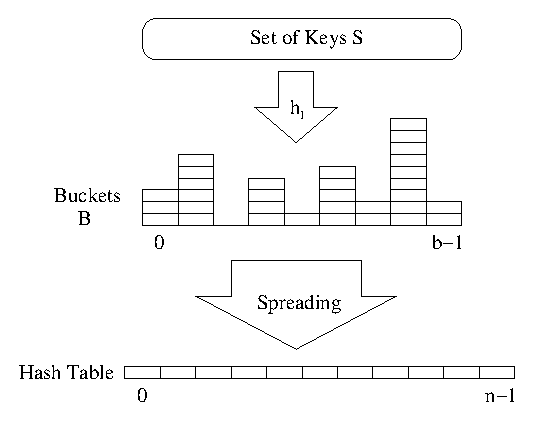
\includegraphics{figs/brz}%
\end{picture}%
\setlength{\unitlength}{4144sp}%
%
\begingroup\makeatletter\ifx\SetFigFont\undefined%
\gdef\SetFigFont#1#2#3#4#5{%
  \reset@font\fontsize{#1}{#2pt}%
  \fontfamily{#3}\fontseries{#4}\fontshape{#5}%
  \selectfont}%
\fi\endgroup%
\begin{picture}(3704,2091)(1426,-5161)
\put(2570,-4301){\makebox(0,0)[lb]{\smash{{\SetFigFont{7}{8.4}{\familydefault}{\mddefault}{\updefault}0}}}}
\put(2782,-4301){\makebox(0,0)[lb]{\smash{{\SetFigFont{7}{8.4}{\familydefault}{\mddefault}{\updefault}1}}}}
\put(2996,-4301){\makebox(0,0)[lb]{\smash{{\SetFigFont{7}{8.4}{\familydefault}{\mddefault}{\updefault}2}}}}
\put(4060,-4006){\makebox(0,0)[lb]{\smash{{\SetFigFont{7}{8.4}{\familydefault}{\mddefault}{\updefault}Buckets}}}}
\put(3776,-4301){\makebox(0,0)[lb]{\smash{{\SetFigFont{7}{8.4}{\familydefault}{\mddefault}{\updefault}${\lceil n/b\rceil - 1}$}}}}
\put(4563,-3329){\makebox(0,0)[lb]{\smash{{\SetFigFont{7}{8.4}{\familydefault}{\mddefault}{\updefault}Key Set $S$}}}}
\put(2009,-3160){\makebox(0,0)[lb]{\smash{{\SetFigFont{7}{8.4}{\familydefault}{\mddefault}{\updefault}0}}}}
\put(2221,-3160){\makebox(0,0)[lb]{\smash{{\SetFigFont{7}{8.4}{\familydefault}{\mddefault}{\updefault}1}}}}
\put(4315,-3160){\makebox(0,0)[lb]{\smash{{\SetFigFont{7}{8.4}{\familydefault}{\mddefault}{\updefault}n-1}}}}
\put(1992,-5146){\makebox(0,0)[lb]{\smash{{\SetFigFont{7}{8.4}{\familydefault}{\mddefault}{\updefault}0}}}}
\put(2204,-5146){\makebox(0,0)[lb]{\smash{{\SetFigFont{7}{8.4}{\familydefault}{\mddefault}{\updefault}1}}}}
\put(4298,-5146){\makebox(0,0)[lb]{\smash{{\SetFigFont{7}{8.4}{\familydefault}{\mddefault}{\updefault}n-1}}}}
\put(4546,-4977){\makebox(0,0)[lb]{\smash{{\SetFigFont{7}{8.4}{\familydefault}{\mddefault}{\updefault}Hash Table}}}}
\put(1441,-3616){\makebox(0,0)[lb]{\smash{{\SetFigFont{7}{8.4}{\familydefault}{\mddefault}{\updefault}Partitioning}}}}
\put(1441,-4426){\makebox(0,0)[lb]{\smash{{\SetFigFont{7}{8.4}{\familydefault}{\mddefault}{\updefault}Searching}}}}
\put(1981,-4786){\makebox(0,0)[lb]{\smash{{\SetFigFont{5}{6.0}{\familydefault}{\mddefault}{\updefault}MPHF$_0$}}}}
\put(2521,-4786){\makebox(0,0)[lb]{\smash{{\SetFigFont{5}{6.0}{\familydefault}{\mddefault}{\updefault}MPHF$_1$}}}}
\put(3016,-4786){\makebox(0,0)[lb]{\smash{{\SetFigFont{5}{6.0}{\familydefault}{\mddefault}{\updefault}MPHF$_2$}}}}
\put(3826,-4786){\makebox(0,0)[lb]{\smash{{\SetFigFont{5}{6.0}{\familydefault}{\mddefault}{\updefault}MPHF$_{\lceil n/b \rceil - 1}$}}}}
\end{picture}%
\vspace{-1mm}
\caption{Main steps of our algorithm}
\label{fig:new-algo-main-steps}
\vspace{-3mm}
\end{figure}

The partitioning step takes a key set $S$ and uses a universal hash function 
$h_0$ proposed by Jenkins~\cite{j97} 
%for each key $k \in S$ of length $|k|$ 
to transform each key~$k\in S$ into an integer~$h_0(k)$.
Reducing~$h_0(k)$ modulo~$\lceil n/b\rceil$, we partition~$S$ into $\lceil n/b
\rceil$ buckets containing at most 256 keys in each bucket (with high
probability).  

The searching step generates a MPHF$_i$ for each bucket $i$, 
$0 \leq i < \lceil n/b \rceil$.
The resulting MPHF $h(k)$, $k \in S$, is given by
\begin{eqnarray}\label{eq:mphf}
h(k) = \mathrm{MPHF}_i (k) + \mathit{offset}[i], 
\end{eqnarray}
where~$i=h_0(k)\bmod\lceil n/b\rceil$.
The $i$th entry~$\mathit{offset}[i]$ of the displacement vector
$\mathit{offset}$, $0 \leq i < \lceil n/b \rceil$, contains the total number
of keys in the buckets from 0 to $i-1$, that is, it gives the interval of the
keys in the hash table addressed by the MPHF$_i$.  In the following we explain
each step in detail.



